\section*{Appendix}


\section{Notations}\label{sec:notation}

This section summarizes all notations used throughout this paper. 

% \begin{table}[h]
% \centering
% \small
% \setlength{\tabcolsep}{8pt}
% \begin{tabular}{l l}
% \toprule
% \textbf{Notations} & \textbf{Definitions or Descriptions} \\ 
% \midrule
% % \multicolumn{2}{l}{\textbf{Dialogue / Data}}\\
% $\mathcal{D}_n=\{(q_t,a_t)\}_{t=1}^n$ & Dialogue prefix of $n$ turns (user $q_t$, model $a_t$) \\
% $q_{\le t}$ & Full history up to turn $t$: $\{q_1,a_1,\dots,q_{t-1},a_{t-1},q_t\}$ \\
% $T_0$ & \# initial turns used for mining/adaptation ($\mathcal{W}$) \\
% $\mathcal{B}$ & Replay buffer of $(q_{\le t}, a_t^F)$ pairs \\
% \midrule
% % \multicolumn{2}{l}{\textbf{Models / Spaces}}\\
% $F,\;G$ & Original (large, black-box) and surrogate (small) models \\
% $\mathcal{M}$ & A generic model; $\mathcal{M}(q_{\le t})=a_t$ \\
% $h_t=f_{\mathcal{M}}(q_{\le t})\in\mathbb{R}^d$ & Hidden state at turn $t$ \\
% $\mathcal{H}_k=\{h_1,\dots,h_k\}$ & Hidden states for first $k$ turns \\
% $\mathcal{M}_k^{T},\;\mathcal{M}_k^{S}$ & Teacher / student local response manifolds \\
% $p_F(\cdot\mid q_{\le t}),\;p_G(\cdot\mid q_{\le t};\theta)$ & Next-token distributions (teacher / student) \\
% $a_t^F,\;a_t^G$ & Text responses from $F$ and $G$ at turn $t$ \\
% \midrule
% % \multicolumn{2}{l}{\textbf{Soft Prompts \& LoRA}}\\
% $P\in\mathbb{R}^{L\times d}$ & Soft prompt  \\
% $\{P_j\}_{j=1}^{k}$ & Bank of $k$ mined soft-prompt directions \\
% $\tilde{s}=V(P)$ & Verbalized prompt sent to black-box teacher $F$ \\
% $\Theta_{\text{LoRA}}$ & Trainable LoRA parameters attached to $G$ \\
% $r_{\text{LoRA}}$ & LoRA rank (e.g., $2\!-\!8$) \\
% \midrule
% % \multicolumn{2}{l}{\textbf{Vocab / Embeddings}}\\
% $\mathcal{V}$ & Student tokenizer vocabulary \\
% $E\in\mathbb{R}^{d\times|\mathcal{V}|}$ & Student embedding matrix; $e_v$ is column for token $v$ \\
% $y_t$ & Teacher token at decoding step $t$ \\
% $\mathcal{N}_k(y_t)$ & Semantic neighborhood of $y_t$ (top-$k$ by cosine in $E$) \\
% $\pi_G(\cdot\mid P,q_{\le t})$ & Student token distribution under prompt $P$ \\
% $\bar e_t = E^\top \pi_G(\cdot\mid P,q_{\le t})$ & Student expectation embedding at step $t$ \\
% $\phi(\cdot)$ & Frozen sentence encoder for fast semantic similarity \\
% \midrule
% % \multicolumn{2}{l}{\textbf{Objectives / Scores}}\\
% $D(\cdot\|\cdot)$ & Distributional divergence (e.g., KL) \\
% $\widehat{D}_t$ & Fast semantic switch score at turn $t$ \\
% $\mathcal{L}_{\text{mine}}$ & Mining loss (semantic unlikelihood + weights) \\
% $\mathcal{L}_{\text{KD}}$ & Black-box KD loss for LoRA distillation (NLL on teacher text) \\
% $\mathcal{L}_{\text{sem}}$ & Semantic alignment: $1-\cos(\phi(a_t^F),\phi(a_t^G))$ \\
% $\mathcal{L}_{\text{stab}}$ & Stability: $\mathrm{KL}(p_G^{\text{pre}}\|p_G^{\text{post}})$ \\
% $w_t$ & Expectation-space weight for step $t$ \\
% \midrule
% % \multicolumn{2}{l}{\textbf{Switching / Drift}}\\
% $m$ & Switch window length (consecutive turns) \\
% $\varepsilon,\varepsilon'$ & Switch threshold and watchdog threshold \\
% $\tau_{\text{drift}}$ & Topic-drift threshold (embedding-space) \\
% \midrule
% % \multicolumn{2}{l}{\textbf{Theory / Complexity}}\\
% $\rho$ & Locality radius of admissible context perturbations \\
% $L$ & Lipschitz constant (local smoothness) \\
% $r$ & Effective rank of teacher–student discrepancy \\
% $\{\lambda_i\}$ & Eigenvalues of discrepancy Fisher / spectrum \\
% $N=k\,T_0\,B$ & Sample count in local KD ($B$ teacher samples per direction) \\
% $\sigma^2$ & Noise proxy for black-box KD / estimator \\
% $\mathcal{R}(\Theta)$ & Capacity/regularization term for tuned params \\
% $\gamma(\rho,L)$ & Local smoothness term in error bound \\
% \bottomrule
% \end{tabular}
% \caption{Notations used throughout this paper.}\label{tab:notations}
% % Scalars are lowercase (e.g., $n$), vectors bold lowercase (e.g., $\boldsymbol{\theta}$), matrices bold uppercase (e.g., $\mathbf{W}$), and sets calligraphic (e.g., $\mathcal{D}_n$).
% \end{table}

\begin{table}[h]
\centering
\caption{Notation summary.}
\label{tab:notation}
\setlength{\tabcolsep}{6pt}
\begin{tabular}{@{}ll@{}}
\toprule
Symbol & Meaning \\
\midrule
$\mathcal{D}_k$ & Dialogue prefix $\{(q_t,a_t)\}_{t=1}^k$ \\
$q_{\le t}$ & Full history up to turn $t$ \\
$F,\,G$ & Original (large) model; surrogate (small) model \\
$S_t$ & \rev{Dialogue state $\mathcal D_{t-1}\oplus q_t$ at turn $t$} \\
$\mathcal{Q}_k$ & \rev{Distribution of later dialogue states after $\mathcal{D}_k$ (local region)} \\
$\mathcal{V}$, $E$ & $G$’s vocabulary; embedding matrix $E\in\mathbb{R}^{d\times|\mathcal{V}|}$ \\
$\Pi_t$ & Next-token distribution of $G$ at turn $t$; entry $\Pi_t[v]$ \\
$\mathbf{e}_v$ & Embedding of token $v$ (column of $E$) \\
$\mathbf{P}\in\mathbb{R}^{L\times d}$ & Soft prompt (row-wise prompt tokens in embedding space) \\
$N_k(u)$ & $k$ nearest neighbors of token $u$ by cosine in $E$ \\
$\overline{\mathbf{e}}_{t,i}$ & Expected embedding $\overline{\mathbf{e}}_{t,i}=E^\top \Pi_{t,i}$ at position $i$ \\
$w_{t,i}$ & Expectation-weighted factor for semantic divergence loss \\
$\mathsf{Gap}_G(S)$ & \rev{Response discrepancy $1-\cos(\phi(a^G(S)),\phi(a^F(S)))\in[0,1]$} \\
$r_t$ & \rev{Anchoring score of warm-start turn $t$ (residual mining loss)} \\
$|B|_{\mathrm{eff}}$ & Effective batch size \rev{$|B|/(m+1)$ under $m$-dependence} \\
$\widehat{\mathsf G}_B$ & \rev{Average gap of the adapted surrogate on a held-out acceptance batch} \\
\bottomrule
\end{tabular}
\end{table}

\section{Related Work}\label{sec:related}

\textbf{Efficient LLM for Multi-turn Dialogues.} Recent efforts to improve multi-turn LLM serving efficiency fall into two main paradigms. The first involves \textbf{single-model approaches} that reduce context length or reuse computation. These include \textit{summarization and context compression}~\citep{wang2025recursively, chen2024compress, xiao2024efficient}, \textit{memory augmentation}~\citep{melz2023enhancing, gutierrez2024hipporag}, and \textit{caching and attention reuse}, \rev{such as CachedAttention~\citep{gao2024cost}, prompt caching~\citep{anthropic_prompt_caching_2024}, resource-aware multi-turn scheduling~\citep{jeong2025accelerating}, isolated per-turn KV compression in FlowKV~\citep{liu2025flowkv}, and adaptive prefill sparsification with progressive KV compression in LoopServe~\citep{li2025loopserve}}. While effective in lowering per-turn cost, these methods still rely on repeated large-model inference, which also leads to high API expenses, latency, and GPU demand. Moreover, they may truncate or underutilize dialogue context, harming performance on complex tasks. The second paradigm adopts \textbf{multi-model approach}, using smaller models for simple queries and escalating difficult ones to larger LLMs~\citep{behera2025towards, schick2023toolformer, ding2024hybrid}, typically via model routing~\citep{shnitzer2023large, ong2024routellmlearningroutellms}\rev{, multi-round routing and aggregation learned with reinforcement learning~\citep{zhang2025routerr1},} and distillation~\citep{hinton2015distilling}. However, pre-trained small models often generalize poorly on complex multi-turn dialogues, while switching models adds inefficiency. 

\rev{\textbf{Relation to systems-level serving and test-time adaptation.} Prefix and KV caching (CachedAttention, prompt caching, FlowKV, LoopServe) reduce the prefill cost of re-processing the history on the \emph{same} large model; the per-token decode cost, memory footprint, and API price of that model are unchanged. SOMA is orthogonal: after the switch it removes the large model from the serving path, and the surrogate can itself be served with prefix caching. Our efficiency comparison already serves every method, including Original, through vLLM with automatic prefix caching enabled (Section~\ref{sec:exp}), so the reported token and latency gains are measured on top of KV-cache reuse. Test-time adaptation methods such as Temp-LoRA~\citep{wang2024templora} and StreamAdapter~\citep{muhtar2024streamadapter} adapt a model to its \emph{own} generated or in-context text; History-FT and SOMA instead perform cross-model distillation, adapting the surrogate to the large model's warm-start responses within the session.}
% Furthermore, recent studies show that LLMs overly rely on early conversational turns~\citep{xiao2023efficient, laban2025llms}, making it harder to maintain coherence and reasoning quality in extended dialogues.


\textbf{Local Manifold Approximation.}  
\rev{We use ``local manifold approximation'' in the informal sense of classical local methods such as LLE~\citep{roweis2000nonlinear}, LTSA~\citep{zhang2007linear}, and Laplacian eigenmaps~\citep{belkin2003laplacian}: a dialogue prefix induces a local region of dialogue states, and SOMA approximates the large model only within that region rather than globally. SOMA does not compute intrinsic dimensions, tangent spaces, or geodesics, and it does not match the hidden spaces of the two models. The local view enters the method only through the output-space discrepancy of Problem~\ref{prob:lma}, which compares responses through a shared sentence encoder, and through the locality gate. Its measurable prediction, that warm-start supervision transfers to later turns until the topic shifts, is tested empirically in Section~\ref{sec:exp} and Appendix~\ref{sec:app_switch}.}

\section{Reproducibility}
In this section, we introduce the details of the experiments in this
paper for reproducibility. At the same time, we have uploaded all necessary code to our GitHub repository to reproduce the results presented in this paper: 
\url{https://anonymous.4open.science/r/SOMA-4175}
. All major experiments are encapsulated as shell scripts, which can be conveniently executed. We introduce the details for reproducibility in the subsections below.

\subsection{Real-World Datasets}\label{sec:app_dataset}

In this section, we briefly present the real-world datasets used in this paper, and all these datasets are commonly used datasets in multi-turn conversation tasks. \textit{ShareGPT}~\citep{chen2024sharegpt4v} is a large-scale collection of high-quality image–text conversations and captions. \textit{ReMeDi}~\citep{yan2022remedi} is a multi-domain Chinese medical dialogue corpus of doctor–patient conversations. \textit{Craigslist}~\citep{he2018decoupling} contains multi-turn buyer–seller negotiation chats from Craigslist, enabling study of bargaining strategies and goal-directed dialogue. \textit{Multi-Char}~\citep{agentlans_multi-character_dialogue_2024} provides multi-character conversational scenarios with role specifications to evaluate coordination and role consistency in multi-party dialogue. \textit{MATH}~\citep{hendrycks2021measuring} is a benchmark of competition-style math problems with step-by-step solutions designed to assess mathematical reasoning in language models. \textit{MT-Bench}~\citep{zheng2023judging} is a multi-turn benchmark to assess response quality across diverse tasks. In this study, we filter out the non-context-dependent dialogues in these datasets. 
% All these datasets are implemented based on Torchvision 0.17.1~\cite{torchvision2016}.
% ShareGPT~\citep{chen2024sharegpt4v}, ReMeDi~\citep{yan2022remedi}, Craigslist~\citep{he2018decoupling}, Multi-Char~\citep{agentlans_multi-character_dialogue_2024}, MATH~\citep{hendrycks2021measuring}, and MT-Bench~\citep{zheng2023judging}

\subsection{Implementation of SOMA}\label{sec:app_implementation}

We implement SOMA based on PyTorch with HuggingFace Transformers, serve inference via vLLM with FlashAttention~\citep{shah2024flashattention}, and run on \rev{Nvidia A6000 GPUs}. Soft–prompt tuning optimizes only the prompt tensor $\mathbf{P}\!\in\!\mathbb{R}^{L\times d}$ on the surrogate $G$ using AdamW, cosine decay, gradient clipping, \rev{and a single forward pass per warm-start turn and step}. The objective combines unlikelihood on a semantic neighborhood, an expectation–weighted penalty using the truncated top–$m$ expectation, and a light anti-degeneration entropy term. \rev{The warm-start context--response pairs, weighted by their anchoring scores $r_t$,} are then used to adapt $G$ with LoRA on \rev{attention and MLP} projections (rank $r$), keeping the base weights frozen; \rev{early stopping is triggered when the training loss stops improving, since all warm-start turns are used for adaptation}. At inference, a cosine closeness gate with a lightweight sentence encoder decides a one–time switch to the adapted surrogate. \rev{All hyperparameters below, including $W$, $|B|$, $M$, and $(k,m)$, are set empirically within the listed ranges; the bounds in Section~\ref{sec:theory} describe how the required margins scale but are too loose at these sample sizes to set them directly.} Prompt length $L\!\in\!\{4, 8,16,32,64\}$; learning rate $\eta\!\in\![1\!\times\!10^{-4},\,5\!\times\!10^{-3}]$; AdamW weight decay $\lambda_{\mathrm{wd}}\!\in\![0,\,10^{-2}]$; gradient clip $\in[0.5,\,1.0]$; neighborhood size $k\!\in\!\{20,50,100\}$; expectation truncation $m\!\in\!\{50,100,200\}$; temperature $\tau\!\in\![0.4,\,1.2]$; expectation weight $\lambda\!\in\![0.5,\,2.0]$; anti–degeneration weight $\beta\!\in\![0.02,\,0.15]$; LoRA rank $r\!\in\!\{4, 8,16,32\}$ with scale $\alpha_{\text{lora}}\!\in\!\{4, 8,16,32\}$; LoRA LR $\eta_{\text{lora}}\!\in\![5\!\times\!10^{-5},\,2\!\times\!10^{-3}]$; warm–start window $W\!\in\![3,\,12]$ turns; acceptance batch $|B|\!\in\![6,\,24]$ contexts; parallel candidates $M\!\in\!\{3,4,5\}$; switch threshold $\varepsilon\!\in\![0.05,\,0.12]$ with $m_{\text{cons}}\!\in\!\{2,3\}$. 
% These choices keep computation modest while aligning with the theory–driven bounds used in the paper.


\subsection{Implementation of Baselines}\label{sec:app_baseline}

\textbf{Original}: We query the large model (family-appropriate: LLaMA-3.1-70B or Qwen-3-8B) with the full dialogue history at every turn to get the responses.

\textbf{Surrogate}: We query the small model (LLaMA-2-7B or Qwen-3-0.6B) with the full dialogue history at every turn to get the responses.

\textbf{History-Prefix}: The surrogate receives the entire conversation produced by the Original up to $t{-}1$ and generates $a_t$; no parameter updates are performed. The switching is the same as SOMA.

\textbf{History-FT}: We fine-tune the surrogate on $(S_t, a_t^{F})$ pairs where $S_t$ is the Original’s full context up to $t$ and $a_t^{F}$ is the next reply, using LoRA on attention projections with early stopping; inference then runs the fine-tuned surrogate without the Original. The switching is the same as SOMA.

\textbf{LLMLingua-2}~\citep{pan2024llmlingua}: We compress the Original’s history at each turn with LLMLingua-2 and feed the compressed summary to the surrogate; we follow the authors’ recommended settings.

\textbf{RouteLLM}~\citep{ong2024routellmlearningroutellms}: We adopt the released router to choose between the Original and the surrogate per turn (complex vs.\ simple queries), following the original settings from the paper.

\subsection{Data Filtering}\label{sec:app_filter}

To ensure that SOMA is evaluated on context-dependent dialogues, we prompt multiple strong LLMs, including GPT-OSS, DeepSeek-V3, and Gemma-2-27B, with the classification prompt shown in Figure~\ref{fig:context_filter}, and retain only conversations that all three models recognize as context-dependent. This avoids model-specific biases and yields a high-quality subset of dialogues where later turns meaningfully depend on earlier turns, matching the use cases in this paper.

\begin{figure}[t]
    \centering
    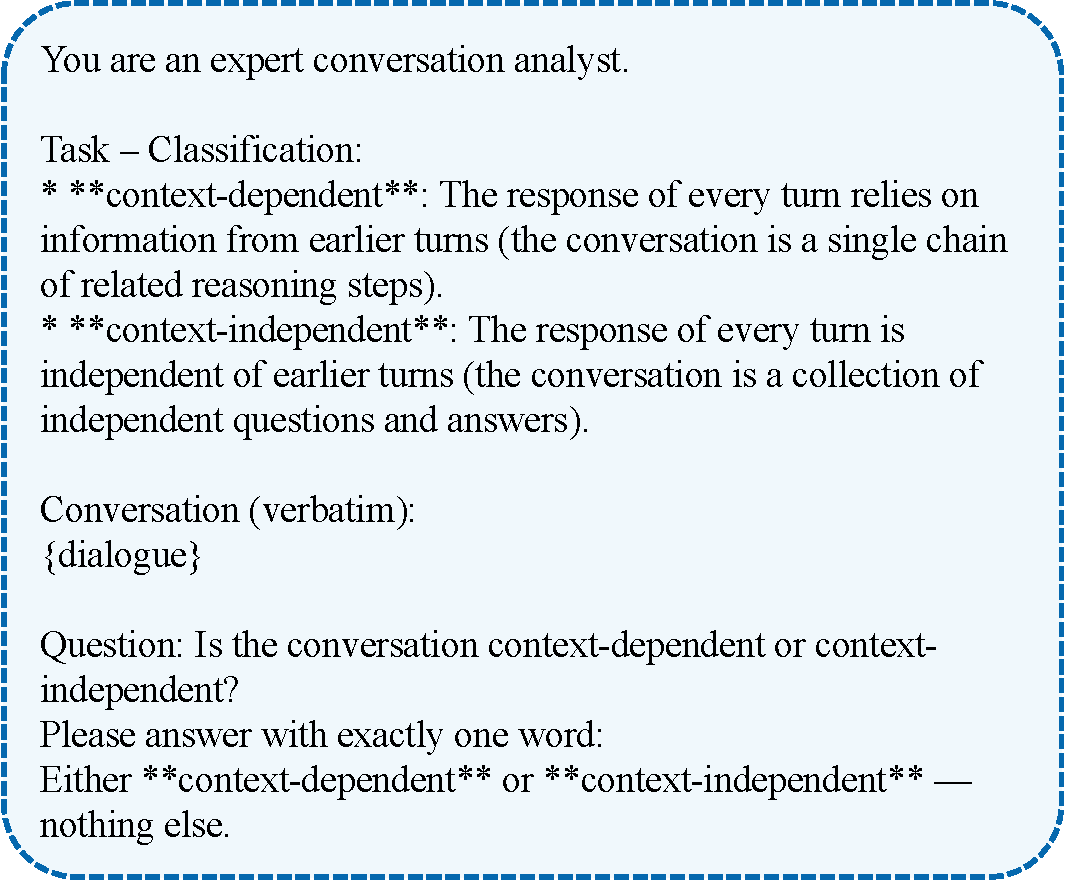
\includegraphics[width=0.8\linewidth]{figure/context_filter.pdf}
    \caption{Instructions for the LLM to filter context-dependent dialogue.}
    \label{fig:context_filter}
\end{figure}

\subsection{Implementation of LLM Judge}\label{sec:app_judge}

The prompt for the LLM judge is shown in Figure~\ref{fig:LLM_judge}. \rev{It adapts the single-answer grading protocol of MT-Bench~\citep{zheng2023judging} and MT-Bench-101~\citep{bai2024mt} to reference-based similarity scoring: the judge receives the original model's response as the reference and scores the surrogate's response on a 0--1 scale along accuracy, reasoning, context integration, and communication. The reference-based framing and the 0--1 scale are our modifications; the MT-Bench protocols grade single answers on a 1--10 scale without a reference. Each response is scored by three judges (GPT-OSS, DeepSeek-V3, and Gemma-2-27B), and we report the mean.}

\begin{figure}[t]
    \centering
    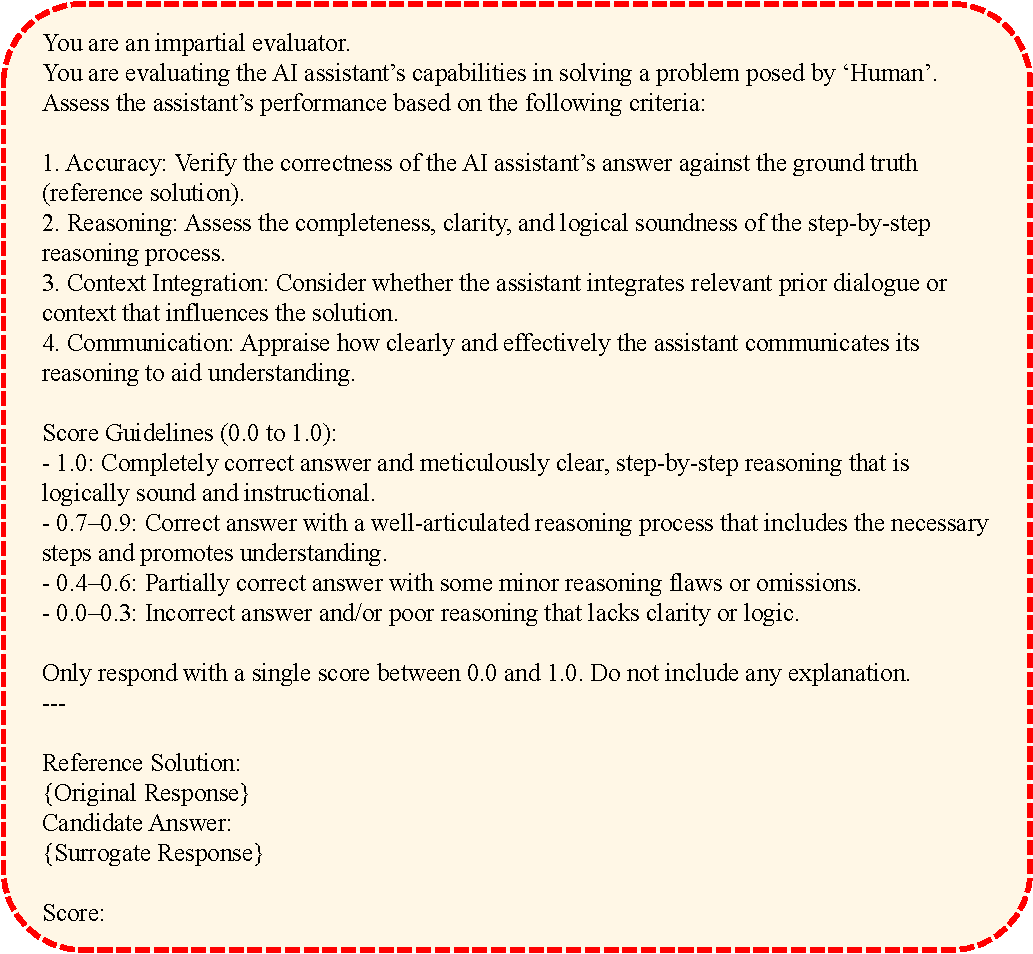
\includegraphics[width=0.8\linewidth]{figure/judge.pdf}
    \caption{Instructions for the LLM judge to evaluate the response similarity.}
    \label{fig:LLM_judge}
\end{figure}

\subsection{Packages Required for Implementation}\label{sec:app_packages}
We perform all experiments on a server equipped with Nvidia A6000 GPUs. Below we list the key packages and their versions used in our implementation:

\begin{itemize}
  \item \textbf{Python} == 3.10
  \item \textbf{pytorch} == 2.8.0 \,+\, CUDA 12.8
  \item \textbf{torchvision} == 0.19.0
  \item \textbf{torchaudio} == 2.8.0
  \item \textbf{numpy} == 1.26.x
  \item \textbf{pandas} == 2.2.x
  \item \textbf{scipy} == 1.12.x
  \item \textbf{cmake} == 3.28+
  \item \textbf{ninja} == 1.11+
  \item \textbf{ipython} == 8.x
  % \item \textbf{jupyter\_core} == 5.x \quad \textbf{jupyter\_client} == 8.x
  \item \textbf{psutil} == 5.9+
  \item \textbf{vllm} == 0.10.2
  \item \textbf{transformers} == 4.56.1
  \item \textbf{accelerate} == 1.9.0
  \item \textbf{bitsandbytes} == 0.46.1
  \item \textbf{sentencepiece} == 0.2.0
  \item \textbf{tiktoken} == 0.11.0
  \item \textbf{einops} == 0.8.1
  \item \textbf{datasets} == 4.0.0
  \item \textbf{huggingface-hub} == 0.34.2
  \item \textbf{safetensors} == 0.5.3
  \item \textbf{ray} == 2.49.1
  \item \textbf{scikit-learn} == 1.7.1
  % \item \textbf{seaborn} == 0.13.2
  \item \textbf{fastapi} == 0.116.2
  \item \textbf{uvicorn} == 0.35.0
\end{itemize}




\section{Mathematical Concepts}\label{sec:app_math}

Here we provide a more comprehensive view of the
relevant concepts that can be helpful to understand the idea of stratification as discussed in the main
body of the paper.

\begin{definition}[Preimage]
Let $f : X \mapsto Y$ be a function from a set $X$ (\emph{domain}) to a set $Y$ (\emph{codomain}). For any subset $N \subseteq Y$, the \emph{preimage} of $N$ under $f$, denoted $f^{-1}(N)$, is defined as:
\[
f^{-1}(N) = \{ x \in X \mid f(x) \in N \}.
\]
\end{definition}
In other words, $f^{-1}(N)$ consists of all elements in the domain $X$ that are mapped into the subset $N$ of the codomain $Y$, regardless of whether every element of $N$ has a preimage.

\begin{definition}[Metric Space]
A set \( X \), whose elements are called points, is said to be a \emph{metric space} if for any two points \( p, q \in X \), there is an associated real number \( d(p, q) \), called the \emph{distance} from \( p \) to \( q \), such that the following three conditions hold:
\begin{enumerate}
    \item \( d(p, q) \geq 0 \), and \( d(p, q) = 0 \iff p = q \);
    \item \( d(p, q) = d(q, p) \) (symmetry);
    \item \( d(p, q) \leq d(p, r) + d(r, q) \) for any \( r \in X \) (triangle inequality).
\end{enumerate}
Any function satisfying these properties is called a \emph{distance function}, or a \emph{metric}.
\end{definition}

\begin{definition}[Neighborhood]
Let \( X \) be a metric space. A set \( N_r(p) \subset X \) is called a \emph{neighborhood} of a point \( p \in X \) if it consists of all points \( q \in X \) such that \( d(p, q) < r \) for some radius \( r > 0 \). The number \( r \) is called the \emph{radius} of the neighborhood.
\end{definition}


\begin{definition}[Continuous]
Let $X$ and $Y$ be two topological spaces. A function $f : X \mapsto Y$ is \emph{continuous} if for each point $x \in X$ and each neighborhood $N$ of $f(x)$ in $Y$, the set $f^{-1}(N)$ is a neighborhood of the point $x \in X$ in the domain.
\end{definition}

\begin{definition}[Topological Equivalence or Homeomorphism]
A function $h : X \mapsto Y$ is called a \emph{homeomorphism} if it is one-to-one, continuous, and has a continuous inverse function. When such a function exists, $X$ and $Y$ are called \emph{homeomorphic} (or \emph{topologically equivalent}) spaces.
\end{definition}

\begin{definition}[Open Set]
A subset \( U \subseteq X \) is called an \emph{open set} if for every point \( p \in U \), there exists a neighborhood \( N_r(p) \subseteq U \). That is, each point in \( U \) has some "wiggle room" around it that still lies entirely within the set \( U \) itself.
\end{definition}

\begin{definition}[Countable Base (Second Countability)]
Let \( X \) be a topological space. A collection \( \mathcal{B} \) of open subsets of \( X \) is called a \emph{base} (or \emph{basis}) for the topology on \( X \) if for every open set \( U \subseteq X \) and every point \( x \in U \), there exists a set \( B \in \mathcal{B} \) such that
\[
x \in B \subseteq U.
\]

If there exists a base \( \mathcal{B} \) that is \emph{countable}, then the space \( X \) is said to be \emph{second countable} or to have a \emph{countable base}; Euclidean spaces, with balls of rational radii around rational points, are a standard example.
\end{definition}

\begin{definition}[Hausdorff Space]
A topological space with the property that two distinct points can always be surrounded by disjoint open sets is called a \emph{Hausdorff space}.
\end{definition}

Essentially, Hausdorff spaces are the spaces where any two points being ``far off'' is defined.

\begin{definition}[Manifold]
A \emph{manifold} of dimension \( n \) is a second-countable Hausdorff topological space in which each point has a neighborhood homeomorphic to Euclidean space \( \mathbb{R}^n \).
\end{definition}

\begin{definition}[Smooth Manifold]
A \emph{smooth manifold} is a manifold \( \mathcal{M} \) equipped with a collection of coordinate charts (i.e., homeomorphisms \( \varphi: U \to \mathbb{R}^n \) for open sets \( U \subseteq \mathcal{M} \)) such that all \emph{transition maps} between overlapping charts,
\[
\varphi_j \circ \varphi_i^{-1} : \varphi_i(U_i \cap U_j) \rightarrow \varphi_j(U_i \cap U_j),
\]
are infinitely differentiable (i.e., \( C^\infty \)). This structure is known as a \emph{smooth atlas}, and it allows calculus to be performed on the manifold.
\end{definition}

\section{Theoretical Results and Proofs}\label{sec:app_proof}

\rev{This appendix states and proves the results used in Section~\ref{sec:theory}. Each statement lists its assumptions, and Section~\ref{sec:warm-start} discusses where our implementation departs from them.

\textbf{Dependence and effective sample size.}
Consecutive dialogue turns are not independent. We assume that the per-turn statistics $Z_1,\ldots,Z_N$ form an $m$-dependent sequence, that is, $\{Z_s\}_{s\le t}$ and $\{Z_s\}_{s>t+m}$ are independent for every $t$, and we define the effective sample size $N_{\mathrm{eff}}=N/(m+1)$; independent samples correspond to $m=0$. For such sequences Hoeffding's inequality holds with $N$ replaced by $N_{\mathrm{eff}}$: if each $Z_s$ takes values in an interval of length $R$, then for every $u>0$
\[
\Pr\Big(\frac1N\sum_{s=1}^{N}\big(Z_s-\mathbb E Z_s\big)\ge u\Big)\le\exp\Big(-\frac{2N_{\mathrm{eff}}\,u^2}{R^2}\Big),
\]
and the same bound holds for the lower tail. This follows from Janson's inequality for sums of partly dependent variables~\citep{janson2004large}, applied to the dependency graph of the sequence, whose fractional chromatic number is at most $m+1$.

\textbf{Locality premise.}
The results below compare statistics measured on warm-start turns with their expectations over the later turns of the session. We therefore assume, as in Section~\ref{sec:prelim}, that warm-start states and later states share the marginal distribution $\mathcal Q_k$. This is the premise that the locality gate monitors and that Figures~\ref{fig:operating}(c) and~\ref{fig:app_switching} test; otherwise they describe only the warm-start distribution.

\bigskip
\textbf{Switching Criterion: Warm-Start Concentration and Acceptance}

\begin{lemma}[Warm-Start Concentration]\label{lem:warmstart}
Let $h(S)\in[0,1]$ be a local statistic that is fixed before the window is observed, such as $\mathsf{Gap}_{\Theta}(S)$ for a fixed adapter $\Theta$ or the distance of a query to a fixed centroid. Let $h(S_1),\ldots,h(S_W)$ be $m$-dependent with common mean $h^\star=\mathbb E_{S\sim\mathcal Q_k}[h(S)]$, and write $\hat h_W=\frac1W\sum_{t=1}^{W}h(S_t)$. Then, with probability at least $1-\delta$,
\[
\big|\hat h_W-h^\star\big|\le\eta_W(\delta):=\sqrt{\frac{\log(2/\delta)}{2W_{\mathrm{eff}}}} .
\]
\end{lemma}

\paragraph{Proof of Lemma~\ref{lem:warmstart}.}
Apply the $m$-dependent Hoeffding inequality with $R=1$ to each tail at level $\delta/2$. Setting $\exp(-2W_{\mathrm{eff}}u^2)=\delta/2$ gives $u=\eta_W(\delta)$, and a union bound over the two tails gives the claim.
\hfill$\square$

\paragraph{Statement: Proposition~\ref{thm:detection}.}
Let the adapter $\Theta$ be fixed given the adaptation data, and let the acceptance batch $B=\{S_1,\ldots,S_{|B|}\}$ be disjoint from that data and drawn from $\mathcal Q_k$ as an $m$-dependent sequence. Let $\widehat{\mathsf G}_B=\frac1{|B|}\sum_{j}\mathsf{Gap}_{\Theta}(S_j)$ and $\mathsf G^\star=\mathbb E_{S\sim\mathcal Q_k}[\mathsf{Gap}_{\Theta}(S)]$. Then, with probability at least $1-\delta$,
\[
\mathsf G^\star\le\widehat{\mathsf G}_B+\gamma_B(\delta),\qquad \gamma_B(\delta)=\sqrt{\frac{\log(1/\delta)}{2|B|_{\mathrm{eff}}}} .
\]
In particular, if $\widehat{\mathsf G}_B\le\varepsilon-\gamma_B(\delta)$, then $\mathsf G^\star\le\varepsilon$ with probability at least $1-\delta$.

\paragraph{Proof of Proposition~\ref{thm:detection}.}
Condition on the adaptation data. Because $B$ is disjoint from it, $\Theta$ is fixed, and $\mathsf{Gap}_{\Theta}(S_1),\ldots,\mathsf{Gap}_{\Theta}(S_{|B|})$ are $m$-dependent with mean $\mathsf G^\star$ and range $R=1$. The lower-tail inequality gives $\Pr(\widehat{\mathsf G}_B-\mathsf G^\star\le-u)\le\exp(-2|B|_{\mathrm{eff}}u^2)$, and setting the right-hand side to $\delta$ gives $u=\gamma_B(\delta)$. On the complementary event, $\mathsf G^\star<\widehat{\mathsf G}_B+\gamma_B(\delta)\le\varepsilon$ if $\widehat{\mathsf G}_B\le\varepsilon-\gamma_B(\delta)$.
\hfill$\square$

\textbf{When the acceptance batch is reused.}
If $B$ overlaps the adaptation data, $\Theta$ depends on the $S_j$ in $B$. The gaps then no longer have mean $\mathsf G^\star$ given $\Theta$, $\widehat{\mathsf G}_B$ is biased downward by the fit, and Proposition~\ref{thm:detection} does not apply. Our implementation reuses the warm-start turns in this way (Appendix~\ref{sec:app_rationale}); holding out part of the warm-start window would restore the bound at the cost of fewer adaptation examples. The bound is also loose at the sample sizes used here: for $\delta=0.05$, $m=0$, and $|B|=24$, $\gamma_B=0.25$, which already exceeds the thresholds $\varepsilon\in[0.05,0.12]$. It therefore describes how the required margin scales with $|B|_{\mathrm{eff}}$ rather than setting the thresholds.

\begin{corollary}[Switching Rule]\label{cor:switch}
Let the locality statistic $h$ satisfy the conditions of Lemma~\ref{lem:warmstart}, and let $B$ satisfy those of Proposition~\ref{thm:detection}. If $\widehat{\mathsf G}_B\le\varepsilon-\gamma_B(\delta)$ and $\hat h_W\le\tau-\eta_W(\delta)$, then, with probability at least $1-2\delta$, both $\mathsf G^\star\le\varepsilon$ and $h^\star\le\tau$.
\end{corollary}

\paragraph{Proof of Corollary~\ref{cor:switch}.}
By Lemma~\ref{lem:warmstart}, $h^\star\le\hat h_W+\eta_W(\delta)\le\tau$ with probability at least $1-\delta$. By Proposition~\ref{thm:detection}, $\mathsf G^\star\le\varepsilon$ with probability at least $1-\delta$. A union bound shows that both hold with probability at least $1-2\delta$.
\hfill$\square$

\bigskip
\textbf{Coverage and Suboptimality to Determine the Number of Soft-Prompt Candidates}

Assume that the mining objective is locally quadratic with curvature $\mathbf H_T\succeq 0$ whose top eigenvector $\boldsymbol v_1$ lies in an $r_{\mathrm{act}}$-dimensional active subspace. SOMA draws its $M$ candidate prompts from an isotropic Gaussian, so their projections onto this subspace point in independent, uniformly random directions. The results below bound the probability that one of them starts within angle $\theta$ of $\boldsymbol v_1$, and the fraction of the top curvature that such a direction retains. They concern the initial directions rather than the optimized prompts, and we set $M\in\{3,4,5\}$ empirically (Appendix~\ref{sec:app_implementation}).

\begin{proposition}[Coverage of the Best Local Direction]\label{thm:coverage}
Let $r_{\mathrm{act}}\ge 2$, let $\boldsymbol v_1$ be a unit vector in an $r_{\mathrm{act}}$-dimensional subspace, and draw $\boldsymbol u_1,\ldots,\boldsymbol u_M$ i.i.d.\ from $\mathrm{Unif}(\mathbb S^{r_{\mathrm{act}}-1})$ in that subspace. For $\theta\in(0,\pi/2]$, let
\[
p_{r_{\mathrm{act}}}(\theta)=\Pr\big(\angle(\boldsymbol u_1,\boldsymbol v_1)\le\theta\big)=\tfrac12\,I_{\sin^2\theta}\Big(\tfrac{r_{\mathrm{act}}-1}{2},\tfrac12\Big),
\]
where $I_x(\cdot,\cdot)$ is the regularized incomplete beta function. Then
\[
\Pr\Big(\min_{m\le M}\angle(\boldsymbol u_m,\boldsymbol v_1)\le\theta\Big)=1-\big(1-p_{r_{\mathrm{act}}}(\theta)\big)^M,
\qquad
p_{r_{\mathrm{act}}}(\theta)\ge\frac{(\sin\theta)^{r_{\mathrm{act}}-1}}{(r_{\mathrm{act}}-1)\,\mathrm B\big(\frac{r_{\mathrm{act}}-1}{2},\frac12\big)} .
\]
For example, $p_{r_{\mathrm{act}}}(\pi/2)=1/2$ for every $r_{\mathrm{act}}$. Isotropic Gaussian initializations satisfy the sampling assumption, because the normalized projection of $\mathcal N(\boldsymbol 0,\sigma^2\mathbf I)$ onto a fixed subspace is uniformly distributed on the unit sphere of that subspace.
\end{proposition}

\paragraph{Proof of Proposition~\ref{thm:coverage}.}
\textbf{Step 1: Exact cap probability.}
Write $r=r_{\mathrm{act}}$ and $T=\langle\boldsymbol u_1,\boldsymbol v_1\rangle$. For $\boldsymbol u_1$ uniform on $\mathbb S^{r-1}$, $T$ is symmetric about $0$ and $T^2\sim\mathrm{Beta}(\frac12,\frac{r-1}{2})$, so $1-T^2\sim\mathrm{Beta}(\frac{r-1}{2},\frac12)$. For $\theta\le\pi/2$ we have $\cos\theta\ge0$, hence
\[
\Pr(T\ge\cos\theta)=\tfrac12\Pr(T^2\ge\cos^2\theta)=\tfrac12\Pr(1-T^2\le\sin^2\theta)=\tfrac12\,I_{\sin^2\theta}\big(\tfrac{r-1}{2},\tfrac12\big).
\]

\textbf{Step 2: Lower bound.}
Let $a=(r-1)/2$ and $x=\sin^2\theta$. Since $(1-s)^{-1/2}\ge1$ on $[0,1)$,
\[
I_x\big(a,\tfrac12\big)=\frac{1}{\mathrm B(a,\frac12)}\int_0^x s^{a-1}(1-s)^{-1/2}\,\mathrm ds\;\ge\;\frac{1}{\mathrm B(a,\frac12)}\int_0^x s^{a-1}\,\mathrm ds=\frac{x^{a}}{a\,\mathrm B(a,\frac12)},
\]
so $p_r(\theta)\ge x^{a}/\big(2a\,\mathrm B(a,\frac12)\big)=(\sin\theta)^{r-1}/\big((r-1)\,\mathrm B(\frac{r-1}{2},\frac12)\big)$.

\textbf{Step 3: Independence across $M$ samples.}
The $M$ draws are independent, so none of them falls in the cap with probability $(1-p_r(\theta))^M$, which gives the coverage probability.
\hfill$\square$

\bigskip
\begin{lemma}[Directional Suboptimality]\label{lem:subopt}
Let $\mathbf H_T\succeq 0$ have largest eigenvalue $\lambda_1$ and top eigenvector $\boldsymbol v_1$. For any unit $\boldsymbol{\hat u}$ with $\angle(\boldsymbol{\hat u},\boldsymbol v_1)\le\theta\le\pi/2$,
\[
\boldsymbol{\hat u}^{\!\top}\mathbf{H}_T\boldsymbol{\hat u} \;\ge\; \lambda_1 \cos^2\!\theta,
\qquad
\lambda_1 - \boldsymbol{\hat u}^{\!\top}\mathbf{H}_T\boldsymbol{\hat u} \;\le\; \lambda_1 \sin^2\!\theta.
\]
\end{lemma}

\paragraph{Proof of Lemma~\ref{lem:subopt}.}
Let $\varphi=\angle(\boldsymbol{\hat u},\boldsymbol v_1)\le\theta$ and decompose $\boldsymbol{\hat u}=\cos\varphi\,\boldsymbol{v}_1+\sin\varphi\,\boldsymbol{w}$ with $\|\boldsymbol{w}\|_2=1$ and $\boldsymbol{w}\perp\boldsymbol{v}_1$. Because $\mathbf H_T\boldsymbol v_1=\lambda_1\boldsymbol v_1$, the cross term vanishes, and
\[
\boldsymbol{\hat u}^{\!\top}\mathbf{H}_T\boldsymbol{\hat u}
=
\lambda_1\cos^2\!\varphi
+
\sin^2\!\varphi\sum_{j\ge 2}\lambda_j \langle \boldsymbol{v}_j,\boldsymbol{w}\rangle^2
\;\ge\;
\lambda_1\cos^2\!\varphi\;\ge\;\lambda_1\cos^2\!\theta,
\]
since $\lambda_j\ge 0$ and $\cos^2$ is decreasing on $[0,\pi/2]$. Subtracting from $\lambda_1$ gives the residual bound.
\hfill$\square$

\bigskip
\begin{corollary}[Candidate Budget]\label{col:M}
Under the conditions of Proposition~\ref{thm:coverage}, the coverage probability within angle $\theta$ is at least $1-\delta$ whenever $M\ge\log(1/\delta)\big/\log\big(1/(1-p_{r_{\mathrm{act}}}(\theta))\big)$. Because $\log(1/(1-p))\ge p$, the simpler condition $M\ge(r_{\mathrm{act}}-1)\,\mathrm B\big(\frac{r_{\mathrm{act}}-1}{2},\frac12\big)\log(1/\delta)/(\sin\theta)^{r_{\mathrm{act}}-1}$ also suffices. Together with Lemma~\ref{lem:subopt}, this trades candidate count against the quality of the best direction.
\end{corollary}

\paragraph{Proof of Corollary~\ref{col:M}.}
Coverage fails with probability $(1-p)^M$, where $p=p_{r_{\mathrm{act}}}(\theta)$, and $(1-p)^M\le\delta$ holds if and only if $M\log(1/(1-p))\ge\log(1/\delta)$. The second condition follows from $\log(1/(1-p))\ge p$ and the lower bound on $p$ in Proposition~\ref{thm:coverage}.
\hfill$\square$}


\section{Additional Experimental Results}
\label{sec:app_exp}

This appendix provides supporting results that complement the main experiments: dataset-level token costs, the effect of warm-start length on switching, and the empirical variance concentration behind the switching bound in Section~\ref{sec:warm-start}.

\subsection{Additional Efficiency Results}
\label{sec:app_eff}

The main text reports the amortized break-even analysis and throughput. Here we provide the dataset-level token results for both model families. Figure~\ref{fig:app_token_costs} shows that \rev{SOMA uses the fewest tokens per dialogue on 11 of the 12 dataset--family pairs; the exception is Craigslist with LLaMA, where Original uses 3\% fewer}. The reason is that after switching, SOMA serves later turns with the adapted surrogate and a compressed context rather than repeatedly sending the full growing history. This avoids the large token cost of Original and History-Prefix while retaining stronger response similarity than directly using the unadapted surrogate.

\begin{figure}[t]
  \centering
  \begin{minipage}[t]{0.49\textwidth}
    \centering
    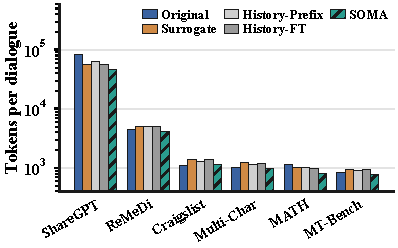
\includegraphics[width=\linewidth]{figure/llama_token_costs.pdf}
    \vspace{-2mm}
    \centerline{\small (a) LLaMA family}
  \end{minipage}\hfill
  \begin{minipage}[t]{0.49\textwidth}
    \centering
    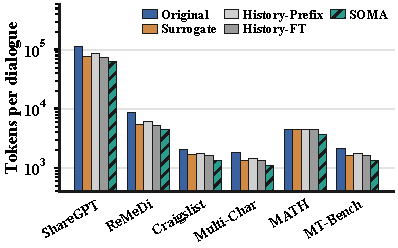
\includegraphics[width=\linewidth]{figure/qwen_token_costs.pdf}
    \vspace{-2mm}
    \centerline{\small (b) Qwen family}
  \end{minipage}
  \vspace{-1mm}
  \caption{Average tokens per dialogue across six datasets. SOMA reduces token usage by avoiding repeated full-history serving after switching.}
  \label{fig:app_token_costs}
\end{figure}

\subsection{Warm-Start Length and Switching Behavior}
\label{sec:app_switch}

The main text (Figure~\ref{fig:app_switching}) reports how final similarity depends on the switch point. The sweep uses warm-start windows \(W\in[1,15]\) and measures the final response similarity after switching. Once the curve flattens, adding more warm-start turns brings little quality gain but delays the efficiency benefit, so short warm starts suffice for general or goal-anchored chats, while compositional reasoning and multi-party dialogues need more evidence before switching.

\subsection{Empirical Variance Concentration}
\label{sec:app_variance}

Finally, we examine how the variance of surrogate--teacher similarity changes with the warm-start window \(W\). For each dataset, we compute the empirical standard deviation across dialogues at each truncation point. Figure~\ref{fig:variance} shows that variance decreases as \(W\) grows: early turns are highly variable, while larger warm-start windows enter a more stable regime. This trend is consistent with the concentration behavior used in Lemma~\ref{lem:warmstart} and the switching bound in \rev{Proposition}~\ref{thm:detection}. In other words, early turns provide the largest information gain, while later warm-start turns mainly reduce uncertainty until the switching decision becomes stable.

\begin{figure}[t]
  \centering
  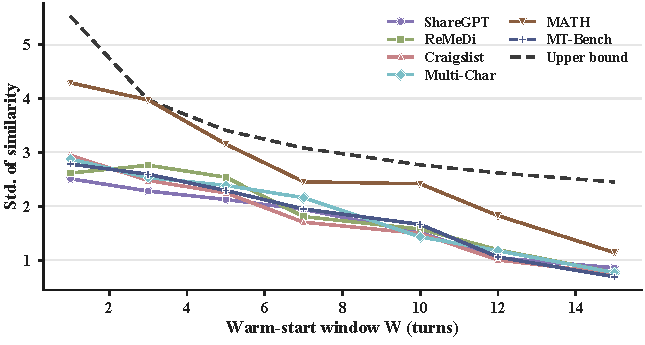
\includegraphics[width=0.78\textwidth]{figure/variance_vs_W.pdf}
  \caption{Variance of response similarity versus warm-start window \(W\). Larger warm-start windows reduce variance and support more stable switching decisions.}
  \label{fig:variance}
\end{figure}


\section{Design Rationale and Serving Considerations}
\label{sec:app_rationale}
\rev{This section collects design questions raised in review that the main text only touches on.

\textbf{Choice of soft prompts and of an adversarial objective.}
Soft prompts are a convenient probe for three practical reasons: they are differentiable, so a handful of gradient steps on the surrogate $G$ can search a continuous neighborhood of the warm-start context instead of enumerating discrete paraphrases; they live in $G$'s own embedding space, so the semantic neighborhood $\mathcal N_k(\cdot)$ and the expected-embedding weight are computed with the same token embeddings and reuse the logits of a single forward pass; and the ANN-based neighborhood keeps the per-step cost proportional to $k+m$ rather than $|\mathcal V|$. Alternative perturbations (input noise, paraphrasing, or adversarial token substitution) can also explore beyond the finite warm-start turns, but they either require an external paraphraser or a discrete search, and they do not directly expose which \emph{directions} in $G$'s input space make $G$ diverge from $F$. We push $G$ away from $F$ rather than toward it because the score must measure how robust the agreement is, not how much agreement a prompt can add. A constructive (divergence-minimizing) prompt would raise the agreement on every turn and yield a signal confounded with the capacity of the prompt itself; an adversarial prompt removes the agreement that is easy to remove, and $r_t$ records what survives. The prompts are then discarded, and only the anchoring scores $r_t$ enter the LoRA objective in Eq.~\ref{eq:lora-ft} as per-turn training weights.

\textbf{Relation to divergence-weighted History-FT and Random-FT.}
The LoRA objective in Eq.~\ref{eq:lora-ft} weights every warm-start turn by its anchoring score $\omega_t\propto r_t$, so SOMA can be read as a weighted History-FT whose weights come from prompt probing rather than from the raw output divergence between $G$ and $F$ on the warm-start turn. The two weightings measure different things and point in opposite directions: raw output divergence emphasizes turns that the \emph{unperturbed} surrogate currently gets wrong, whereas the anchoring score emphasizes turns whose teacher response the surrogate still predicts \emph{after} an adversarial perturbation, i.e., responses that are determined by the dialogue state and hence likely to transfer to later turns. The ablation in Figure~\ref{fig:llama_ablation} isolates the contributions of the mining objective's two terms, but it does not include a baseline that weights History-FT by raw output divergence or one that samples training turns uniformly at random with the same LoRA budget; we consider both key controls and leave them, with a prompt-length sweep, to future work.

\textbf{Robustness, divergence, and the perturbation space.}
We do not prove that robustness under prompt perturbations is a better predictor of adaptation utility than direct output divergence, nor that the continuous perturbation space of $\mathbf P$ covers the space of natural-language future turns. We therefore treat these as modeling assumptions and test them indirectly: the topic-shift stress test (Figure~\ref{fig:operating}(c)) probes future turns that leave the mined region, and the warm-start sweep (Appendix~\ref{sec:app_switch}) shows how much of the local behavior is captured as the window grows. A direct empirical comparison of the two weightings is the most informative next step for validating the mining objective.

\textbf{Number of large-model calls and target consistency.}
The original model $F$ is queried once per warm-start turn to serve the user; these $W$ responses are stored and reused as the mining targets $a_t^F$, as the LoRA targets, and as the references for the acceptance gate. $F$ is not re-queried while $\mathbf P$ is optimized, so the targets are never stale with respect to the dialogue state, and the soft prompt perturbs only the surrogate side of the objective. Because the acceptance gate reuses these turns, the acceptance bound of Section~\ref{sec:warm-start} does not certify the gate as implemented; holding out part of the warm-start window would restore it at the cost of fewer adaptation examples. Prompt mining and LoRA adaptation run entirely on the surrogate and consist of a small number of forward--backward passes over the $W$ warm-start turns ($M$ candidate prompts times the mining iterations, followed by the LoRA steps). Their wall-clock cost is part of the end-to-end latency reported in Figure~\ref{fig:operating}(a).

\textbf{Drift detection.}
The drift statistic is the cosine distance between recent queries and the warm-start centroid, monitored over a sliding window; rollback triggers after $m_{\mathrm{cons}}$ consecutive violations. Because the statistic is continuous, gradual drift raises it progressively rather than only at abrupt shifts, and Corollary~\ref{cor:switch} would bound the probability of accepting a surrogate whose true gap exceeds the margin if the acceptance batch were held out and the centroid fixed in advance. As implemented, both come from the warm-start turns, so the initial switch is a heuristic check (Section~\ref{sec:warm-start}). Re-switching after a rollback differs: its acceptance batch and refreshed centroid come from the turns $F$ serves after the shift, which the adapter never saw, so the held-out condition of Proposition~\ref{thm:detection} holds for that decision. The gate does not certify that the centroid distance tracks every form of quality degradation, which is why we also report the false-rollback and detection rates in Figure~\ref{fig:operating}(c).

\textbf{Serving many session-local adapters.}
A LoRA adapter of rank $r$ on the attention and MLP projections of LLaMA-2-7B has about $2.5r$ million parameters ($\approx 20$M parameters, or roughly 40~MB in bfloat16, for $r=8$), i.e., well under $1\%$ of the surrogate. Multi-adapter serving systems batch requests from many adapters over a single copy of the base weights and page adapters between host and GPU memory~\citep{sheng2023slora}, so GPU residency is bounded by the number of concurrently \emph{switched} sessions rather than by the total number of sessions, and an adapter is discarded as soon as its session ends. The mining and adaptation steps for a session are independent of other sessions and can be scheduled as short background jobs on the surrogate replica. We did not benchmark multi-node concurrent adapter scheduling; the reported latencies are for the single-session serving path described in Section~\ref{sec:method}.}

\section{Broader Impact}
\label{sec:broader_impact}

SOMA aims to reduce the cost and latency of multi-turn LLM serving by replacing repeated large-model inference with session-local surrogate serving. This can make interactive LLM systems more efficient, accessible, and environmentally sustainable. At the same time, using a smaller surrogate may introduce quality degradation if the dialogue leaves the learned local state, especially in high-stakes settings such as medical, legal, or financial assistance. SOMA mitigates this risk through semantic acceptance and drift-aware rollback, but deployment should still include monitoring, conservative thresholds, and human oversight where errors may cause harm. Since SOMA uses dialogue history for local adaptation, practical deployments should also apply data minimization, retention limits, and privacy-preserving processing of the dialogue history.



\section{Limitations and Future Work}
\label{sec:limitations}

SOMA has several limitations. First, the surrogate's capacity limits how closely it can match the original model. When the small--large model gap is very large, some behaviors cannot be recovered by session-local adaptation alone. Second, soft-prompt mining requires access to the surrogate tokenizer and embedding space, which makes SOMA harder to deploy in strict black-box API settings. Third, SOMA is designed for locally coherent dialogues. Abrupt topic changes, noisy warm-start windows, or strong paraphrase shifts can weaken the learned local directions, although the drift gate is designed to reduce persistent degradation. Finally, SOMA introduces a one-time warm-start cost, so it is most suitable for medium-to-long sessions where post-switch savings can amortize the initial adaptation overhead. \rev{Two further limitations concern evaluation. Gradual topic drift is detected by the same continuous centroid statistic as abrupt shifts, but we have only stress-tested abrupt shifts (Figure~\ref{fig:operating}(c)); quality may degrade before the rollback margin is exhausted. We also have not compared SOMA against a History-FT variant weighted by raw output divergence or against uniformly sampled local turns under the same LoRA budget (Appendix~\ref{sec:app_rationale}), so the incremental value of prompt mining over simpler weightings is supported by the component ablation rather than by a direct head-to-head comparison against these alternatives.}

Future work can improve SOMA along several directions. Better drift detectors could make rollback more reliable under topic shifts. Approximate mining methods could reduce the need for internal surrogate access. Multi-region adaptation could support conversations with multiple topics, and privacy-preserving mining could make the method safer for sensitive dialogue settings. Another promising direction is to amortize soft-prompt search across related sessions and extend SOMA to multimodal serving, where early turns often carry images or documents.